\documentclass[12pt,letterpaper]{extarticle}

\usepackage{caption} % for the figure captions
\usepackage[osf]{mathpazo} % a nicer font
% this is a package for the citation formats: found this formulation sorted natbib errors when changing packages
%from http://tex.stackexchange.com/questions/54480/package-natbib-error-bibliography-not-compatible-with-author-year-citations
\usepackage[square,sort,comma,numbers]{natbib} 
\usepackage{amsmath} % package for equations
\usepackage{url} % package for urls
\usepackage{hyperref} % for hyperlinks
\usepackage[a4paper, total={6in, 9in}]{geometry}
\hypersetup{
     colorlinks   = true,
     citecolor    = gray
}
\usepackage{graphicx} % for the figures
\usepackage{pdfpages}
\hypersetup{linkcolor=blue}

\pagenumbering{gobble}

\graphicspath{ }

%Title page
%Itinerary
%Localities
%Kit list
%Contact details
%Where staying: all deets

\begin{document}

%title

{\Huge\textbf{\textit{Cheirolepis}}\par}
\vspace{3mm}
{\large{Kye-row-leep-iss} \par} 
\vspace{5mm}
\textit\textit{Cheirolepis} is one of the \textbf{earliest relatives of the living ray-finned fishes}; this is the group that includes almost all living fishes - trout, tuna, goldfishes etc.  Like the rest of our fossils, it is from the Devonian - between 420 and 360 million years ago - of Scotland. \textit{Cheiracanthus} had a mouthful of \textbf{sharp teeth} and would have been a predator in the Devonian waters.  It could have used its large, powerful fins to chase smaller fishy prey. \newline

\begin{figure}[h!]
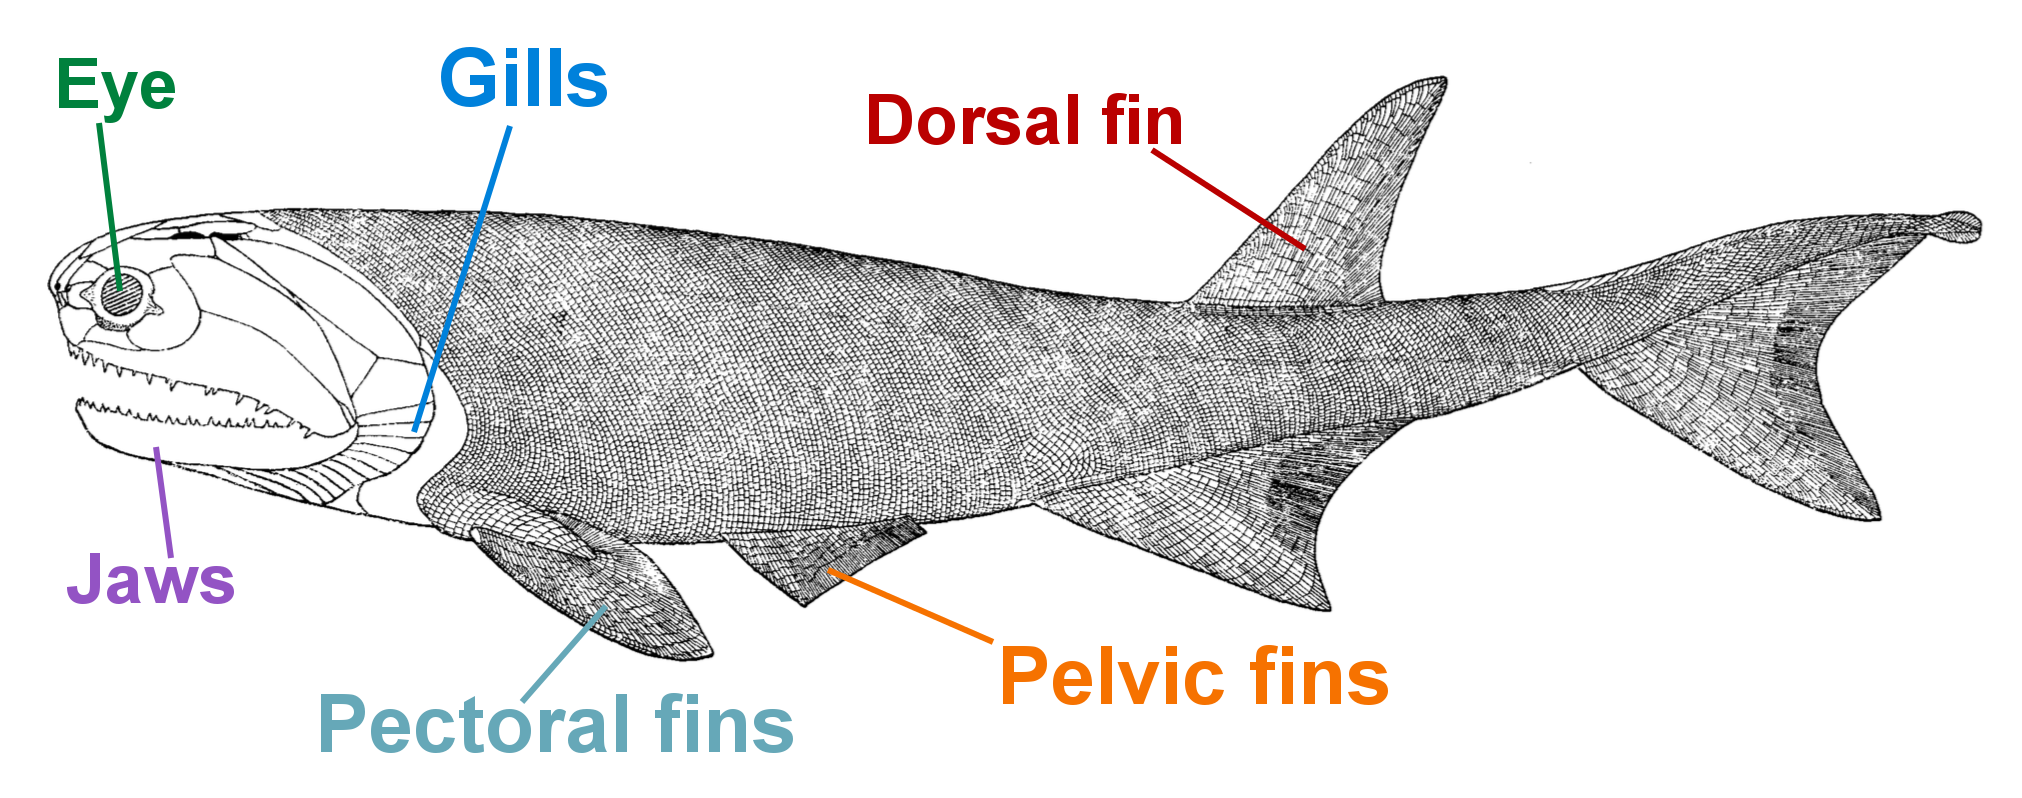
\includegraphics[scale=0.4]{Cheirolepis}
\centering
\end{figure}

{\large\textbf{\underline{Fossil facts}}\par}

\begin{itemize}
  \item If you look at the scales of \textit{Cheirolepis} you'll see they're very small - they're actually more similar to the scales of sharks and acanthodians than to the larger scales of other bony fishes like \textit{Osteolepis} and \textit{Dipterus.}
\end{itemize}


\end{document}